\documentclass{beamer}
\setbeameroption{show notes}

\usepackage[spanish,es-ucroman]{babel}
\usepackage[spanish, backgroundcolor=green]{todonotes}

\usetheme[
    language=spanish,
    titlepagelogo=../paper/latex/Graphics/uhlogo,
    pageofpages=de,
    notshowauthor=true,
    secondlogo=true,
    titleline=false,
    color=red
]{TorinoTh}

\setbeamertemplate{headline}{}

\setrellabel{Tutor}
\setcandidatelabel{Tesista} \setassistentsupervisorlabel{Co Tesis} \setsubject{Tesis}

\titlepagesecondlogo{graphics/matcom-logo}
\title{Sistema de Votaci\'on Representativa sobre \textit{Quorum}}
\author{Andy Ledesma Garc\'ia}
\rel{Yaidir Mustelier Ruiz}
\ateneo{Universidad de La Habana. MATCOM}
\date{13 de diciembre de 2022}  % @remind cambiar si la fecha es otro d\'ia

\begin{document}
\titlepageframe

\begin{frame}
    \frametitle{D\'eficit Fiscal}
    \framesubtitle{Monetizaci\'on vs. Endeudamiento P\'ublico}

    \begin{alertblock}{Problema}
        Los ingresos fiscales resultan insuficientes para financiar la actividad del sector público de un país.
    \end{alertblock}

    \pause

    Soluciones:
    \begin{itemize}[<+->]
        \pause

        \item monetizaci\'on de la deuda p\'ublica
        \note[item]<3>{Los bancos financian la deuda p\'ublica}
        \note[item]<3>{Produce inflaci\'on}
        \item endeudamiento p\'ublico
        \note[item]<4>{el estado se endeuda y promete devolver en un tiempo. El monto y cr\'edito de la deuda se plasman en un doc llamado \textbf{bono soberano}}
    \end{itemize}

    \onslide<5->
    \begin{center}
        \Large \highlightbf{Mercado de Deuda P\'ublica}
    \end{center}
\end{frame}

\begin{frame}
    \frametitle{Obtenci\'on del Prestamista}

    \todo[inline]{@TODO pon foto pa ocupar espacio}
    
    \begin{enumerate}
        \pause

        \item $\text{bono soberano} = \text{monto solicitado} + \text{cr\'edito m\'aximo}$
        \item<5-> confecci\'on de los \highlightbf{Comit\'es de Mercado Financiero} 
        \note<5>{
            \begin{itemize}
                \item autoridad de mercado q regirá el reglamento del MDP
                \item adopta las medidas q estime convenientes
                \item tiene potestad disciplinaria sobre todos los operadores del mercado
                \item para su confecci\'on se realiza un proceso de votaci\'on representativa \todo[inline]{@audit c\'omo se determinan espec\'ificamente los candidatos y el presidente?} 
            \end{itemize}
        }
        \item<3-> subasta 
        \note<3>{se subasta a ver ki\'en pide menos cr\'edito}
        \item<4-> prestamista $=$ ganador
    \end{enumerate}
\end{frame}

\begin{frame}
    \frametitle{Sistema de Votaci\'on Representativa}
    \framesubtitle{Definici\'on y Conteo de Votos}

    \includegraphics<1>{../paper/latex/Graphics/rep-voting.pdf}

    \note<1>{
        \begin{itemize}
            \item el poder de voto es transferible, esto implik q un participante puede ser a la vez votante y candidato
            \item a lo sumo un voto por votante
        \end{itemize}
    }
    \includegraphics<2>{graphics/rep-voting-colored-winner.pdf}

    \note<2>{en este sistema hay dos problemas principales a enfrentar...}
\end{frame}

\begin{frame}
    \frametitle{Sistema de Votaci\'on Representativa}
    \framesubtitle{Ciclos}

    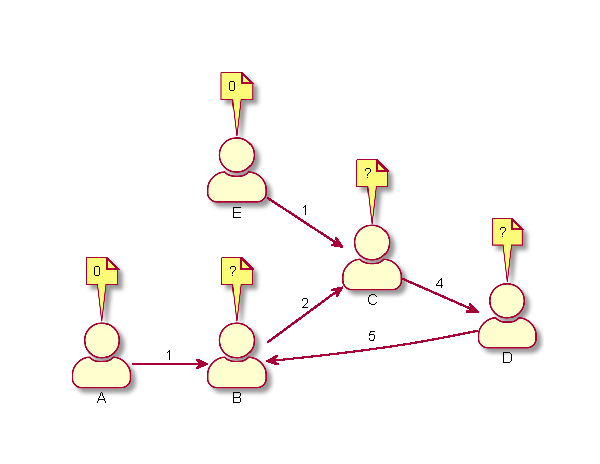
\includegraphics{../paper/latex/Graphics/voting-cycle.pdf}
    \note{no keda claro cu\'antos votos asignar a los del ciclo de manera  justa, de acuerdo con el proceso de votaci\'on}
\end{frame}

\begin{frame}
    \frametitle{Sistema de Votaci\'on Representativa}
    \framesubtitle{Empate en el Primer Lugar}

    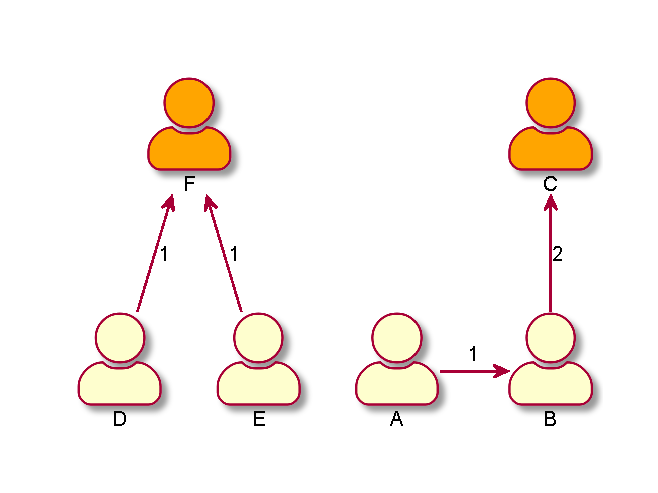
\includegraphics[scale=.9]{graphics/2-winners.pdf}
    \note{
        \begin{enumerate}
            \item hay q seleccionar un solo ganador
            \item s\'olo hay q atender a los empates en el 1er lugar
        \end{enumerate}
    }
\end{frame}

\begin{frame}
    \frametitle{Implementaci\'on en \textit{Quorum}}

    \begin{itemize}
        \item registro perdurable de votos
        \item conteo autom\'atico

        \todo[inline]{@TODO poner todo lo bueno q tiene hacerlo  en quorum y poner pause cada vez q hayas puesto items afines a lo mismo: cosas buenas heredadas de ser un sistema electro'nico, cosas buenas d ser descentralizado, cosas buenas d ser cliente de ethereum...}
    \end{itemize}

\end{frame}

\end{document}